% -------------------------------------------------------
\section{Methodology}
\label{sec:methodology}
% -------------------------------------------------------

\subsection{Dataset and Target Scope}

The dataset is made from gfissore/arxiv-abstracts-2021 on HuggingFace Hub (1,999,486 preprints)\cite{arxiv_abstracts_2021}. To build it, only abstracts where the main category is the first author-assigned field in cs.LG, cs.CL, cs.AI are kept. Papers listed with these categories only as secondary are excluded because their main argument is based on their primary subfield. After requiring abstracts to have at least 50 words and to include both year and category information, 24,677 abstracts remain. For time-based analysis, five-year periods (2000–04 to 2020–21) are used. This is because yearly groups were too small before 2005 (only a few hundred), while ten-year groups would mask the 2014–2015 change observed in the baseline.

\begin{figure}[H]
\centering
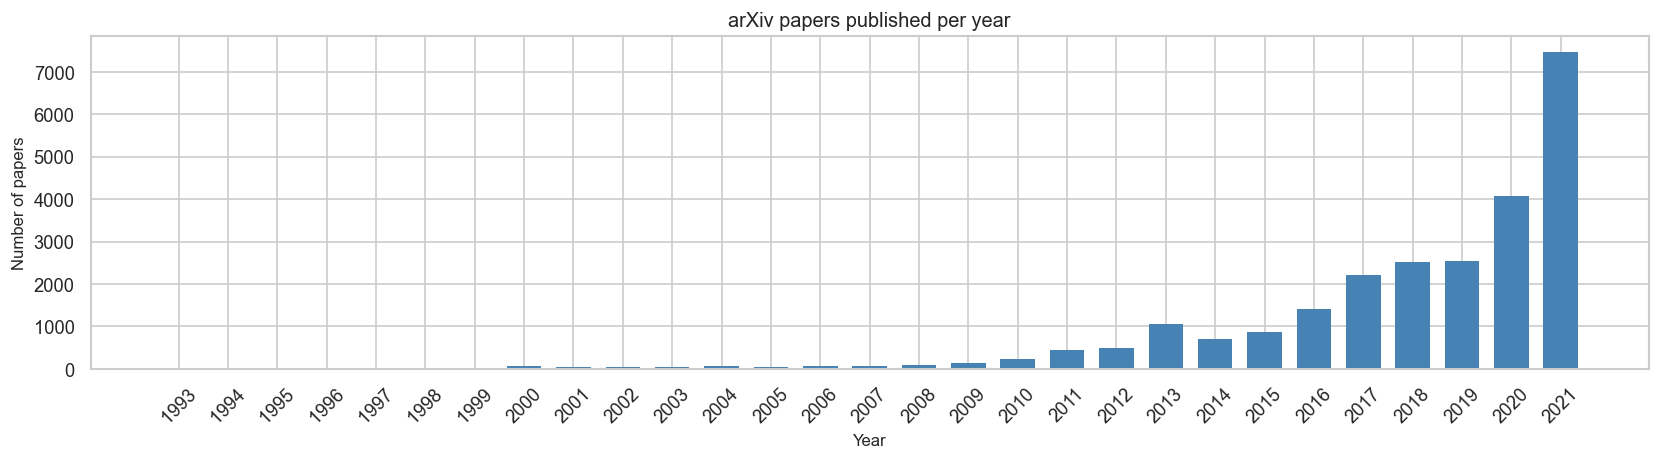
\includegraphics[width=\columnwidth]{figures/eda_figures/fig1a.png}
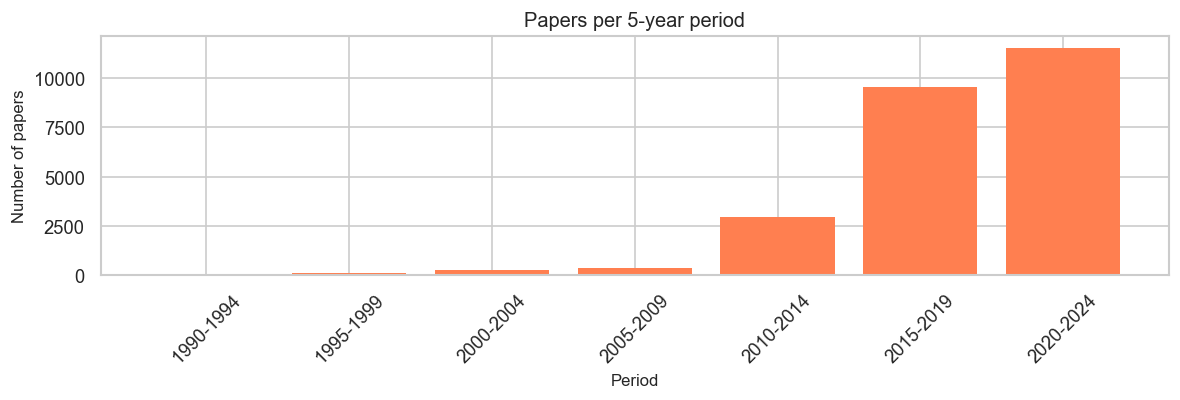
\includegraphics[width=\columnwidth]{figures/eda_figures/fig1b.png}
\caption{Publication volume over time, showing the 27-fold skew from 2000--2004 to 2020--2021 that motivates period-level reliability weighting.}
\label{fig:terminology_diff}
\end{figure}

\subsection{Preprocessing Pipeline}
\begin{center}
\begin{tikzpicture}[
    box/.style={
        draw,
        rounded corners,
        align=center,
        font=\scriptsize,
        minimum width=3.2cm,
        minimum height=0.8cm
    }
]

% Row 1
\node[box, fill=stepblue] (a) {1. Load \\ HuggingFace Dataset};
\node[box, fill=stepblue, right=0.6cm of a] (b) {2. Standardised ID - \\ YY.MM + Stripping Suffix};

% Row 2
\node[box, fill=stepblue, below=0.6cm of a, text width=3.2cm] (c)
{3. Extract Year \\ 
$yy \geq 19 \rightarrow 20yy$ \\ 
$yy < 19 \rightarrow 19yy$};
\node[box, fill=stepblue, right=0.6cm of c] (d) {4. Clean Text \\ ASCII | Punct | Lowercase};

% Row 3
\node[box, fill=steppurple, below=0.6cm of c] (e) {5. Filter Category \\ primary in (cs.LG,cs.CL,cs.AI)};
\node[box, fill=stepblue, right=0.6cm of e] (f) {6. Assign Period \\ 5 year winder (2000-2004...)};

% Row 4
\node[box, fill=stepblue, below=0.6cm of e] (g) {7. Tokenise + Lemmatise \\ NLTK + WordNet + Stopwords};
\node[box, fill=steppurple, right=0.6cm of g] (h) {8. Filter Records \\ 50 tokens, year \& \\ category present};

% Row 5 (final)
\node[box, fill=stepgreen, below=0.6cm of g] (i) {9. Output \\ id.year.title.abstract.cat.period};

% Arrows
\draw[->] (a) -- (b);
\draw[->] (b) -- (c);

\draw[->] (c) -- (d);
\draw[->] (d) -- (e);

\draw[->] (e) -- (f);
\draw[->] (f) -- (g);

\draw[->] (g) -- (h);
\draw[->] (h) -- (i);

\end{tikzpicture}
\end{center}
The preprocessing pipeline is designed to support both traditional bag-of-words models and transformer-based embeddings. For bag-of-words methods, we apply aggressive abstract cleaning to reduce noise and standardise lexical features, whereas raw abstracts are preserved separately for SentenceBERT and SPECTER2 \cite{specter2} to retain semantic richness. Text normalisation includes ASCII filtering, punctuation removal, and lowercasing, followed by tokenisation and WordNet-based lemmatisation to reduce vocabulary sparsity. A domain-specific stopword list of 24 terms (e.g., \textit{paper, study, work, approach, used, based}) is applied in addition to the standard NLTK English stopwords to further eliminate high-frequency academic boilerplate. Finally, records are filtered for minimum content length and completeness, and enriched with structured metadata including temporal periods and category labels for downstream analysis.

\subsection{Text Representations}
Five representations are used across the project; each is chosen to make a different layer of change visible: surface vocabulary, distributional neighbourhood, or full discourse

\begin{table}[H]
\centering
\caption{Representation models and semantic interpretation layers}
\small
\setlength{\tabcolsep}{3pt}

\begin{tabularx}{\columnwidth}{p{2.2cm} p{2.2cm} X}
\toprule
\textbf{Representation} & \textbf{Level} & \textbf{Interpretation / Use} \\
\midrule

BoW (term counts) 
& raw frequency 
& LDA baseline; keyword-frequency model used as a lexical reference \\
\addlinespace

TF-IDF (sublinear) 
& discriminative vocabulary 
& Keyword baseline used in NMF; sensitive to vocabulary choice and PCA-related instability \\
\addlinespace

Word2Vec (skip-gram) 
& local neighbourhood semantics 
& Captures terminology diffusion via co-occurrence drift in embedding space \\
\addlinespace

Sentence-BERT (MiniLM-L6) 
& abstract semantic representation 
& Centroid drift analysis using PCA and UMAP projection of semantic structure \\
\addlinespace

SPECTER2 
& scientific discourse embedding 
& Models terminology diffusion and discourse-level semantic drift across scientific literature \\
\bottomrule
\end{tabularx}
\end{table}

\subsection{Lexical Keyword Analysis (M5)}

The baseline operationalises theoretical versus applied focus as the relative prevalence of two hand-curated keyword sets. An initial vocabulary of 14 theory and 15 application terms was reduced after exploration: high-frequency ambiguous terms such as model, method, results, and framework appeared with nearly equal frequency in both orientations and flattened the signal. The retained sets theory: \{theory, hypothesis, framework, approach, theorem\}; application: \{application, dataset, experiment, implement\} trade coverage for signal clarity. Two scores are computed per year $y$ and keyword set $K$:

{\small
\begin{equation}
\text{RTF}(y, K) = \frac{\sum_{d \in D_y} \sum_{k \in K} \text{count}(k,d)}{\sum_{d \in D_y} |d|_{\text{chars}}}
\end{equation}
}

{\small
\begin{equation}
\text{tfidf}(t,d) = (1 + \log \text{tf}(t,d)) \cdot \log \frac{|D|}{|\{d' : t \in d'\}|}
\end{equation}
}

Character-level normalisation in Eq. 1 was chosen over per-document averaging because post-filter abstract lengths span 50–400 tokens. Sublinear TF in Eq. 2 is essential; without it, near-function terms dominate year-level means. Both representations place the crossover at 2014–2015.

\subsection{Topic Modelling}

Topic modelling removes the closed-vocabulary constraint of the baseline and allows themes to emerge from the data. LDA (Gensim) on a bag-of-words matrix and NMF (scikit-learn) on a TF-IDF matrix were trained and compared for $k \in \{6, 8, 10\}$ topics. Model quality is evaluated with $C_v$ coherence, which tracks co-occurrence of top-weighted words within a sliding reference window and is the standard human interpretability proxy for short-document corpora. Held-out perplexity was deliberately excluded as it rewards diffuse topics and correlates poorly with human judgments on short documents. NMF with $k = 10$ was selected ($C_v = 0.55$ vs.\ $0.48$ for LDA at the same $k$); topics were manually labelled as \textit{theory-oriented} (\texttt{algorithm}, \texttt{optimisation}, \texttt{inference}) or \textit{application-oriented} (\texttt{dataset}, \texttt{healthcare}, \texttt{translation}, \texttt{recommendation}) and aggregated into a time-wise theory/application ratio directly comparable with the lexical baseline.
\subsection{Limitations Framing and Classification}

To check if the type of limitation mentioned in abstracts has changed, keywords were divided into four separate groups:  \textit{failure} (\texttt{fail}, \texttt{degrade}), \textit{capability} (\texttt{cannot}, \texttt{limited}), \textit{hedging} (\texttt{may}, \texttt{could}), and \textit{ethics} (\texttt{bias}, \texttt{fairness}). For each abstract, a yes/no marker shows if any keyword appears in each group, and the average proportion is calculated across groups. Another test uses logistic regression on TF-IDF word features to tell apart 2010–2013 from 2018–2020 abstracts, two separate time periods chosen to avoid confusion from transition years. Five-fold cross-validation is applied; per-class F1 scores are reported along with accuracy because there are more late-period abstracts than early ones, and the confusion matrix is checked for uneven errors, where late abstracts are wrongly labeled as early ones to find leftover early-period words in late abstracts.

\subsection{Representation Geometry and Temporal Drift}

To test whether the shifts identified lexically and thematically leave a geometric trace, each abstract is embedded, and per-year centroids are compared. TF-IDF captures surface vocabulary change; SentenceBERT (\texttt{all-MiniLM-L6-v2}, mean-pooled) captures semantic change. For visualisation, PCA (2D) and UMAP are both applied: PCA preserves global variance while UMAP preserves local neighbourhoods; both are reported because a single projection can mislead. Quantitative drift is computed in full-dimensional space---50-component PCA for TF-IDF and 384-dimensional space for SBERT---because the 2D TF-IDF projection retains only approximately 1.6\% of total variance. Temporal movement is the consecutive year centroid distance:

{\small
\begin{equation}
    d(y) = \| \boldsymbol{\mu}(y) - \boldsymbol{\mu}(y-1) \|, \quad
    \boldsymbol{\mu}(y) = \frac{1}{|D_y|} \sum_{d \in D_y} \phi(d)
    \tag{3}
\end{equation}
}

Series are $[0,1]$-normalised for cross-representation comparison. Robustness is confirmed by near-perfect agreement between Euclidean and cosine distance ($r \approx 1.00$), confirming observed patterns are properties of the representation, not the metric.

\subsection{Terminology Diffusion (M2)}

To follow individual terms through the big change, three matching signals are calculated for each candidate term in each time period. Candidate terms are identified by retaining the top 60 rising TF-IDF terms for each period; about 37\% are removed because they are part of longer phrases, leaving around 48 candidates. Before training Word2Vec, 174 multi-word phrases are combined into single tokens with underscores to avoid incorrect splitting.

\begin{enumerate}[leftmargin=*, label=(\roman*)]
\item \textbf{TF-IDF delta} delta weighted late minus early period mean frequency per 10,000 words measures surface adoption.
\item \textbf{Word2Vec neighbourhood cosine}, calculated between skip-gram models made for each period (vector size 300, window 12, epochs 30), measures how much a term's context changes; the models are aligned using a Procrustes orthogonal transformation based on 1,436 shared anchor terms (6.9\% of the combined vocabulary), with reliability scores of 0.27 and 0.49 for the two earliest periods.
\item \textbf{SPECTER2 discourse drift} (\texttt{allenai/specter2}, HuggingFace) captures argumentative repositioning at the abstract level; embedding operates on raw non-lemmatized abstracts (batch size 64, L2-normalized) with bootstrap aggregation stabilizing small-sample cells.
\end{enumerate}

All three signals are scaled between 0 and 1 and cut off at 0.5 to create a four-part classification that separates terms spreading actively from those copied from templates, where high frequency and almost no change in discourse indicate uniform terminology rather than real idea spread.
